\documentclass{article} 
\usepackage{amsthm}
\usepackage{amsmath}
\usepackage{graphicx}
\usepackage{subfigure}
%\usepackage{subfig}
\usepackage{verbatim}
\newtheorem{theorem}{Theorem}[section]
\newtheorem{corollary}[theorem]{Corollary}
\newtheorem{defination}{Definition}[section]
\begin{document} 
\section{The Collision Probability of Y Set}
\paragraph{Glossary} The symbol, abbreviation and marks needed in
expressing the shift stage and probability computation.

\subsection{Preliminaries}
\paragraph{The Equality of Two Sets}
Assume there are two sets, marked as X\_A and X\_B, having same NO. of elements and the number is M. Each element is given an index from 1 to M. The definition of Identical Index Equality is expressed here:
\begin{defination}
Identical Index Equality(IIE): For any i$\in$[1,M], X\_A[i]=X\_B[i].
\end{defination}
The definition of Cross Index Equality is expressed here:
\begin{defination}
Cross Index Equality(CIE): For any i,j$\in$[1,M], X\_A[i] = X\_B[j], where i$\neq$j
\end{defination}
Any two sets that have same number of elements can be splited into several sub-sets and each sub-sets contains several (X\_A[i],X\_B[i]) pairs. The number of sub-sets various from 1 to M. We give the definition of set level equality of two sets with same number of elements:
\begin{defination}
Set Level Equality(SLE): Each sub-set have one of the two kinds of Equality.
\end{defination}
For two sets X\_A and X\_B, if there is no way of split that at least one sub-set is of CIE and there are at least one way of split that all sub-sets are of IIE, then such X\_A and X\_B are IIE only Sets. 
The definition of CIE only Sets is given in same way.

\subsubsection{Replay Attack and Y Set Collision}
\paragraph{The Message Sets in CETD Under Replay Attack}
\begin{itemize}
	\item D\_A and D\_B are definitely IIE.
	\item X\_A=D\_A, X\_B=D\_B
	\item Y\_A and Y\_B are just SLE
	\item when Y\_A and Y\_B are SLE, tag collision
\end{itemize}
In replay attack, the adversary replace a data-tag pair on the memory with a
pair copied from the same address at an old time point. That means for the two
pairs at different time point, the two message block sets and related tags are
identical respectively, while the nonce N$_A$ and N$_B$ are randomly generated and
the equality is unpredictable if their generator is of high quality.  That means
the shifting bits parameter segment on the nonce R\_A and R\_B, are randomly
generated.

In this scenario, the probability of a successful attack can be expressed as the equation 1.1:
\begin{defination}
Pr[Successful Replay Attack] = Pr[Tag$_a$ = Tag$_b$ $\mid$ (D\_A = D\_B) \& (R\_A and R\_B are random)]
							 = Pr[Y\_A = Y\_B $\mid$ (D\_A = D\_B) \& (R\_A and R\_B are random)]
							 
D\_A and D\_B sets are of Identical Index Equality. Y\_A and Y\_B is of Set Level Equality.
\end{defination} 

We can see that the set level equality of Y\_A and Y\_B will directly leads to the collision of tag and cause the succeed of replay attack. 
For easy understanding, we assume the shuffle stage does not work at first, which means D\_A = X\_A = D\_B = X\_B(IIE). Hence the Y set is the output of rotate shifting stage in CETD, we will analyze the properties of block rotate shifting and the cases of input sets that can result Y set collision(SLE). 

\begin{figure}[htbp]
 \centering
 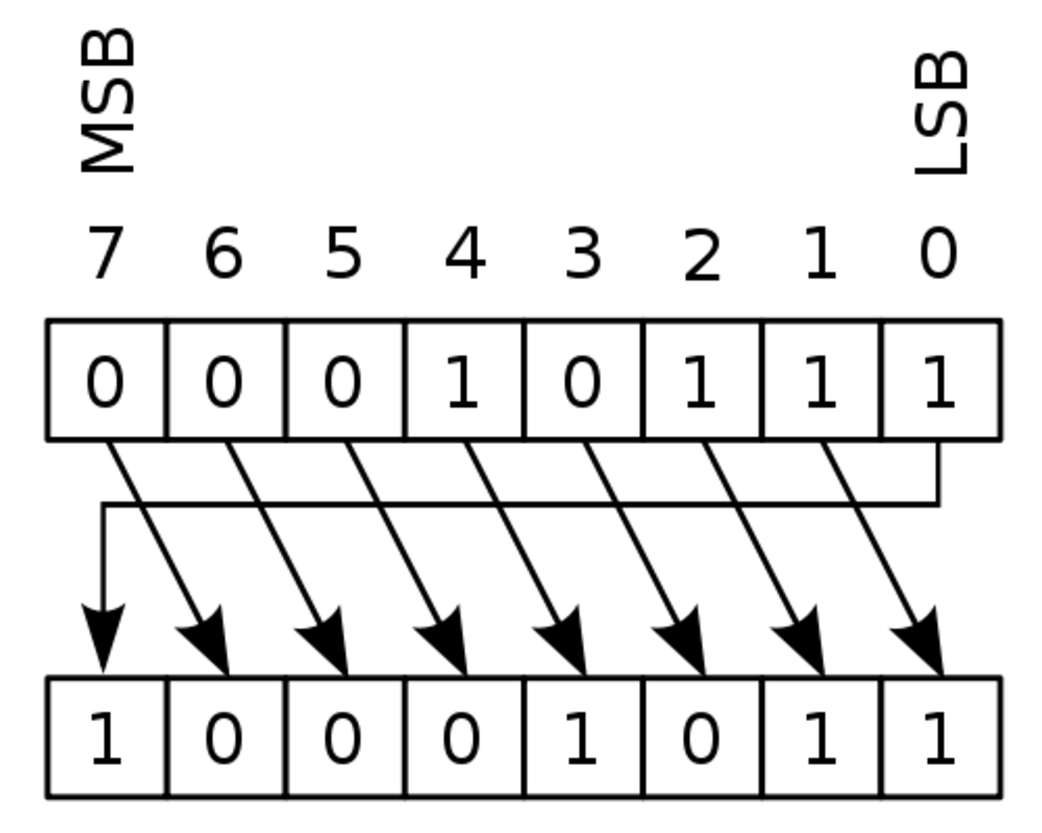
\includegraphics[scale=0.4]{./diagrams/rotate_right.pdf}
 \caption{The Concept of Rotate Shifting(Right)}
 \label{fig:1 }
\end{figure}

\subsubsection{Rotate Shifting Introduction} 
\begin{itemize}
	\item the concept of rotate shift
	\item The examples of X,R,Y
\end{itemize}
Unlike logical shifting and arithmetic shifting, rotate shifting
behaves like whirling a wheel. The empty position in a message block shifted is
filled by the bits shifted out. Figure 1 express the concept of rotate shift.

We can refer that the result of rotate shifting a message block depends on the
value of block and the bits shifted.  If two message blocks whose value are
identical are shifted with distinct R$_i$s, the result blocks may be
identical.That means when R$_i$ fixed,the mapping from message blocks to the
shifted result blocks is not injection. This case is expressed in Figure 2(a).

For two distinct message blocks, however, their result blocks may be identical
when their R$_i$s are distinct. This case is expressed in Figure 2(b).  
When the R$_i$s of two message blocks are identical, the equality of result blocks
is same as the equality of their input blocks.				

\begin{figure}
\centering
\subfigure[Same Block Shifted Different Bits]{
\begin{minipage}[b]{0.45\textwidth}
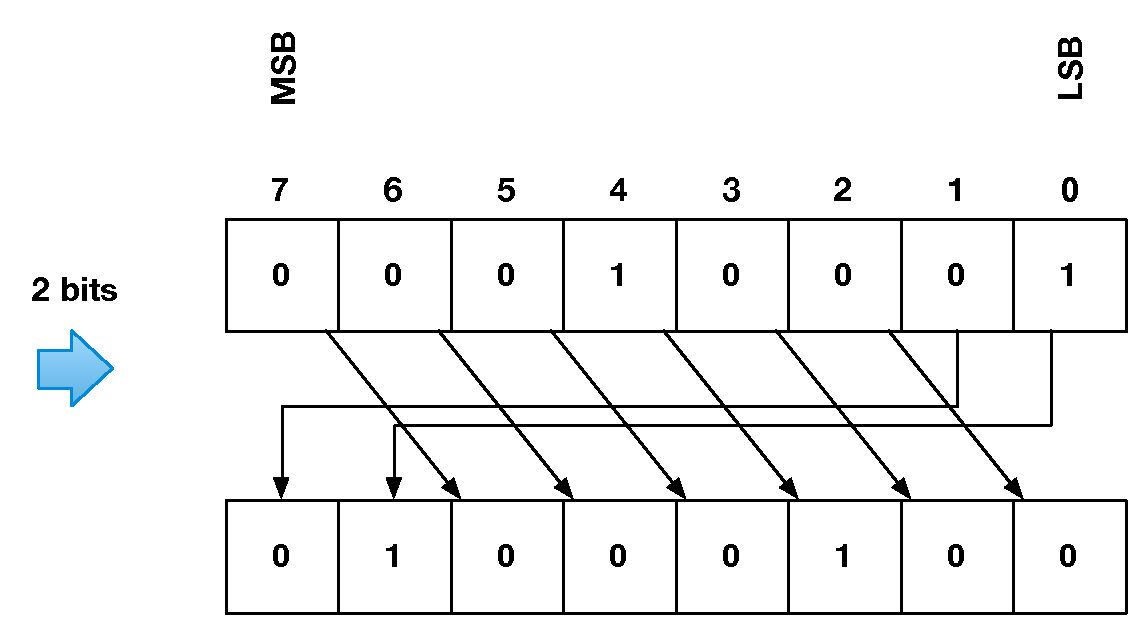
\includegraphics[width=1\textwidth]{./diagrams/r_s_2bits.pdf} \\
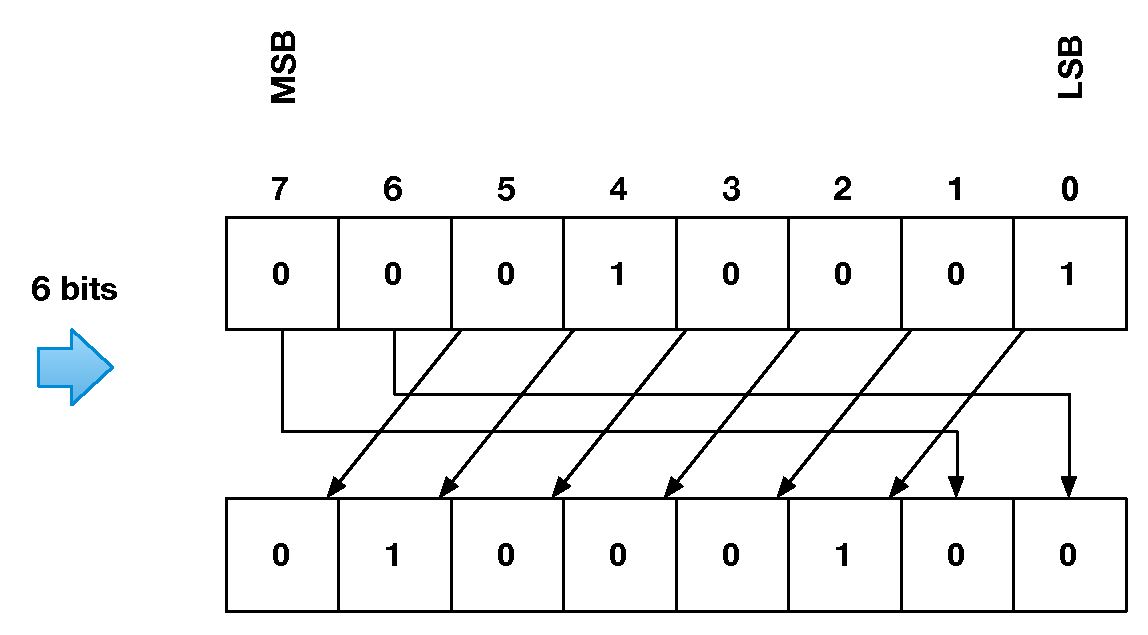
\includegraphics[width=1\textwidth]{./diagrams/r_s_6bits.pdf}
\end{minipage}
}
\subfigure[Different Blocks Shifted Different Bits]{
\begin{minipage}[b]{0.45\textwidth}
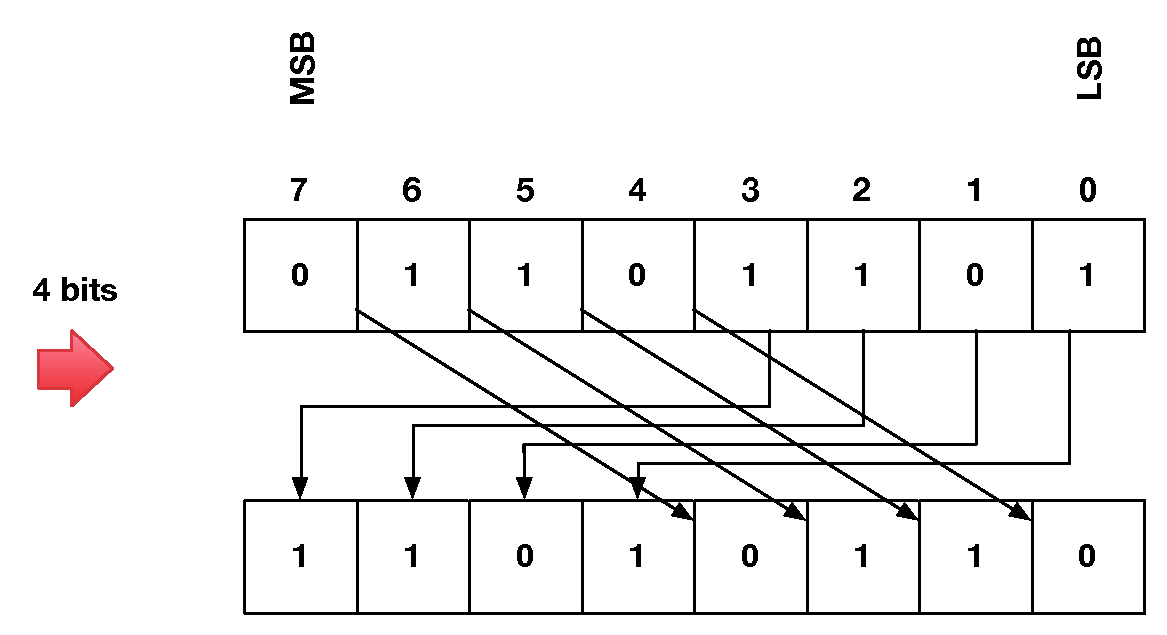
\includegraphics[width=1\textwidth]{./diagrams/r_d_4bits.pdf} \\
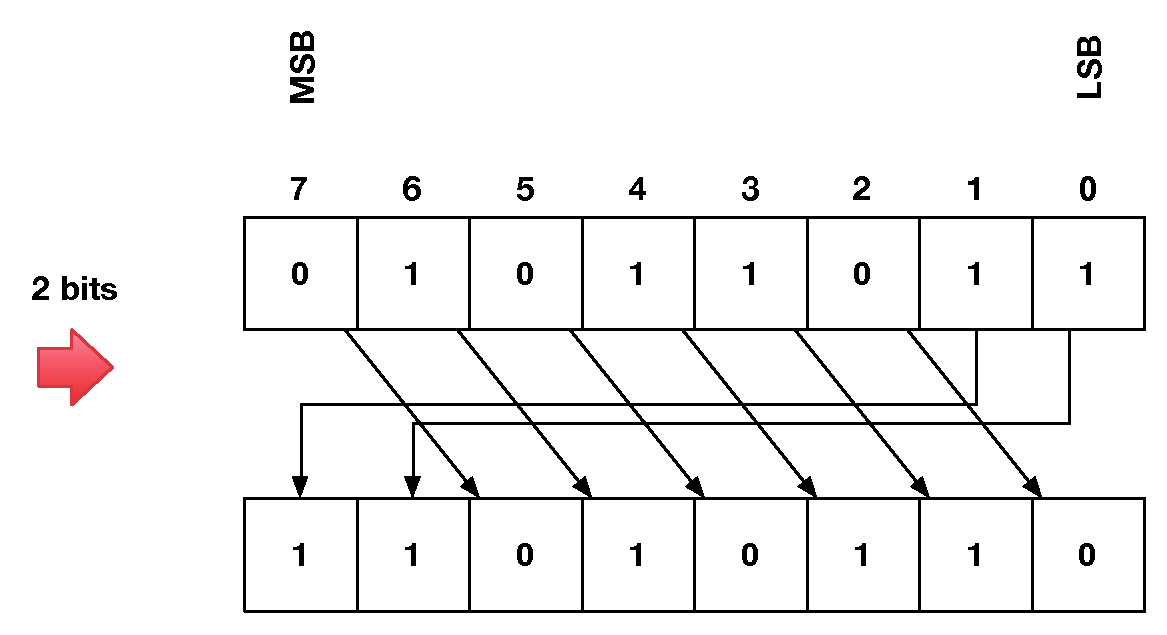
\includegraphics[width=1\textwidth]{./diagrams/r_d_2bits.pdf}
\end{minipage}
}
 \caption{The Examples of Y Block Collision}
 \label{fig:2 }
\end{figure}


\begin{figure}
\centering
\subfigure[Only Single Block Equality]{
 \label{fig:y_single_e} %% label for first subfigure
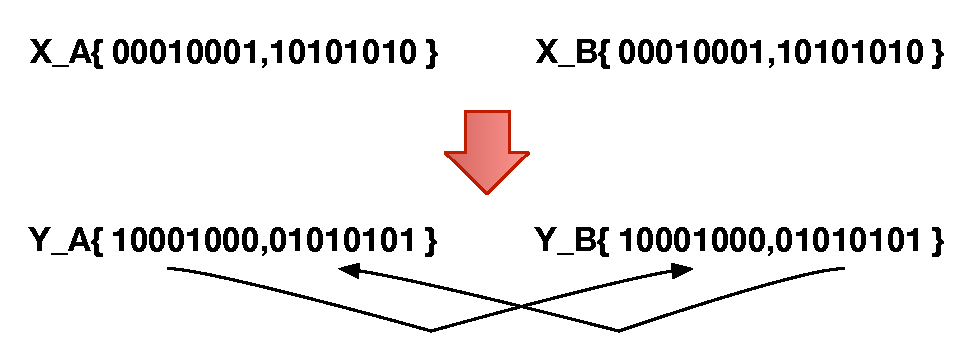
\includegraphics[width=.5\textwidth]{./diagrams/y_single_equality.pdf}
}
%\hspace{1in}
\subfigure[Only Set Level Equality]{
\label{fig:y_set_e} %% label for second subfigure
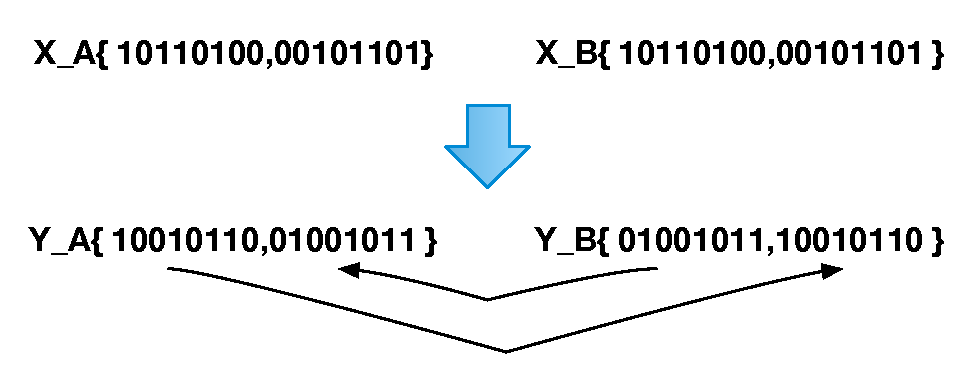
\includegraphics[width=.5\textwidth]{./diagrams/y_set_equality.pdf}
}
\caption{X Set Pairs with Only One Type of Y Equality}
 \label{fig:y_e_single} %% label for entire figure
\end{figure}

\begin{figure}
\centering
\subfigure[Single Block Equality Case]{
 \label{fig:y_both_single} %% label for first subfigure
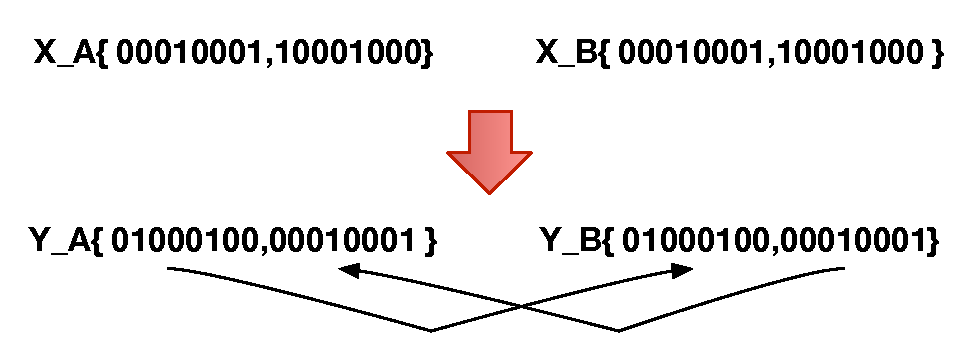
\includegraphics[width=.5\textwidth]{./diagrams/y_both_single.pdf}
}
%\hspace{1in}
\subfigure[Set Level Equality Case]{
\label{fig:y_both_set} %% label for second subfigure
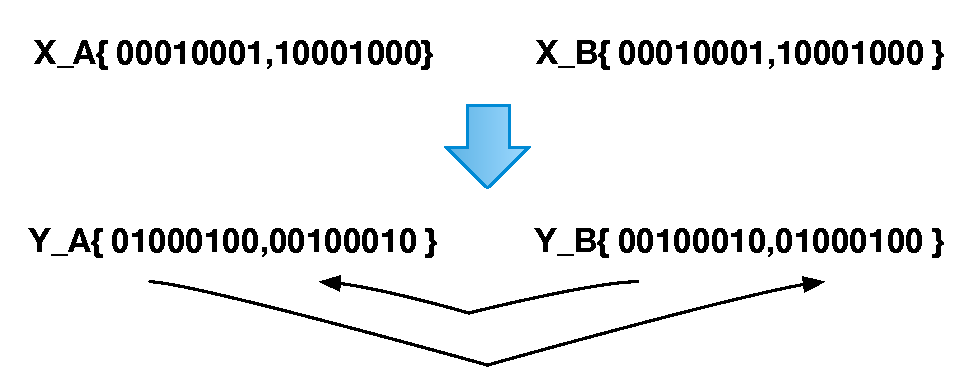
\includegraphics[width=.5\textwidth]{./diagrams/y_both_set.pdf}
}
\caption{A X Set Pair with Two Types of Y Equality}
 \label{fig:y_both} %% label for entire figure
\end{figure}

\subsection{Rotate Shifting and Y Set Collision} 
\begin{itemize}
	\item distinct pairs in R sets: IIE pairs and CIE pairs
	\item X block pairs causing IIE Y block pairs
	\item X block pairs causing CIE Y block pairs
\end{itemize}
Assume the shuffle stage does not work, then D\_A= X\_A=D\_B=X\_B,which means the following properties exist in X\_A and X\_B:
\begin{itemize}
	\item X\_A[i] = X\_B[i] for all i$\in$[1,M], M is the number of elements
	\item The equality of elements in a X set is uncertain.
\end{itemize}
That means X\_A and X\_B are of Identical Index Equality. 
All the analysis in this section is based on the assumption that shuffle stage does not work.
If such X\_A and X\_B result two Y sets of Set Level Equality using two identical shifting bits parameter sets R\_A and R\_B, the the related tag T$_a$ = T$_b$.
 
Figure 3 and Figure 4 express the examples of X sets that lead to SLE Y sets with distinct R sets. In this paper, we analyze the cases of the input set pair (X\_A and X\_B) of shifting stage in CETD under replay attack that can lead to Y set pair collision(SLE).



\subsubsection{Case of X Sets Resulting Y Set Collision}
\begin{itemize}
	\item If R\_A $\neq$ R\_B, there is at least one pair distinct
	\item the related x blocks pairs should generate a SLE y pairs.
	\item if the Y pairs are iie, then each X block pair has pattern
	\item if the Y pairs are cie, then each X block in a sub-set is from a same base
\end{itemize}
Assuem the number of distinct block pairs in R\_A and R\_B is R$_d$. For these R block pairs, their related X\_A and X\_B blocks formed a sub-group, marked as X\_A$_s$ and X\_B$_s$, and this sub-group is IIE. The related sub-group in Y\_A is marked as Y\_A$_s$ and the one in Y\_B for Y\_B$_s$.

\paragraph{Identical Index Equality Case}
As shown in Figure 2(a), two identical X blocks can result two identical Y blocks while their relative shifting bit parameter R[i] and R[j] are distinct. 
We found that the identical X block pair X\_A[i]=X\_B[i] resulting identical Y blocks with distinct R\_A[i] and R\_B[i] have a common property, this property is expressed in Theorem 1.

\begin{theorem}
Assume X\_A[i] and X\_B[i] are two identical block from two set X\_A and X\_B with same index i. X\_A[i] and X\_B[i] have same number of bits N=2$^n$. The result of rotate shifting X\_A[i] and X\_B[i] with distinct shifting bit parameter R\_A[i] and R\_B[i] are marked as Y\_A[i] and Y\_B[i]. Then Y\_A[i] and Y\_B[i] can be identical only when X\_A[i] and X\_B[i] are formed by repeating a binary pattern P, which is a binary segment. The length of this pattern P can be expressed as:

	P\_L = 2$^p$, p$\in$[0,n-1]
\end{theorem}

Assume the two X sets X\_A and X\_B are identical and can  form single block equality. Base on Theorem 1.1, we can conclude the corollary of the relationship between X set pair and Y set pair for single block case. 
\begin{corollary}
Assume there is M elements in X\_A and X\_B. If there is at least one i$\in$[1,M], X\_A[i] = X\_B[i] is formed by repeating a pattern P$_i$ whose length is P\_L$_i$ = 2$^pi$, then Y\_A and Y\_B can be single block identical with some two distinct shifting bits parameter sets R\_A and R\_B.
\end{corollary} 

\paragraph{Cross Index Equality Case}
From Figure 2(b) we can see that two distinct X blocks X\_A[i] and X\_B[j] can result two identical Y blocks Y\_A[i]=Y\_B[j] when the relative R\_A[i] $\neq$ R\_B[j]. 



We found that if Y\_A$_s$ and Y\_B$_s$ are CIE, the related X\_A$_s$ and X\_B$_s$ contains a property. 
This property is expressed in Theorem 2.

\begin{theorem}
Assume X\_A[i] and X\_B[j] are two distinct blocks from two set X\_A and X\_B and i$\neq$j. X\_A[i] and X\_B[i] have same number of bits N=2$^n$. 
The result of rotate shifting X\_A[i] and X\_B[j] with distinct shifting bit parameter R\_A[i] and R\_B[i] are marked as Y\_A[i] and Y\_B[i]. 

Then Y\_A[i] and Y\_B[j] can be identical when X\_A[i] can be rotate shifted to X\_B[i]
\end{theorem}

Assume the two X sets X\_A and X\_B are identical and can form set level equality. Base on Theorem 1.2, we can conclude the corollary of the relationship between X set pair and Y set pair for set level equality. 
\begin{corollary}
Assume there are M elements in X\_A and X\_B. If there is at least two pairs of data, marked as (X\_A[i],X\_B[j]) and (X\_A[j]),X\_B[i]) where i,j$\in$[1,M] and i$\neq$j, that X\_A[i] can be formed by shifting X\_A[j], then Y\_A and Y\_B can be set level identical with some two distinct shifting bits parameter sets R\_A and R\_B.
\end{corollary} 

\paragraph{An Intersection Case}
Base on Corollary 1.3 and Corollary 1.4, we can draw the following corollary for the X set pairs that can form both set level and single block equality:
\begin{corollary}
Assume there is M elements in X\_A and X\_B. If there are at least two pairs of data, marked as (X\_A[i],X\_B[j]) and (X\_A[j]),X\_B[i]) where i,j$\in$[1,M] and i$\neq$j, that X\_A[i] can be formed by shifting X\_A[j] and X\_A[i] = X\_B[i] or X\_A[j]=X\_B[j] is formed by repeating a pattern P$_i$ whose length is P\_L$_i$ = 2$^pi$ , then Y\_A and Y\_B can be either set level or single block identical with some two distinct shifting bits parameter sets R\_A and R\_B.
\end{corollary}
The proof of Theorem 1.1 and Theorem 1.2 and Corollary 1.2 to 1.5 can be refered in appendix.


\subsection{The Probability of Y Set Collision} 
\begin{itemize}
	\item Assume the sub-set contaions M blocks, the probability that they are both pattern 
	\item if they are both pattern, the probability that Y set are iie
	\item the probability that they are from same base
	\item if they are same base, the pro that Y set is cie
	\item the probability that bothe pattern and same base
	\item if both, the pro of Y SLE
\end{itemize}
Hence the shift bit parameter set R\_A and R\_B are randomly generated, the probability of Y set collision for each input case is determined by the number of specific combinations of R\_A and R\_B. The computation of Pr[Y\_A = Y\_B] is based on this idea.

\subsubsection{Single Block Equality Case}
Assume two identical sets X\_A and X\_B satisfy the following properties:
\begin{itemize}
	\item Each element is formed by a pattern with same length P\_L = 2$^p$
	\item Each element cannot be formed by rotate shifting any other element.
\end{itemize}
Such two sets X\_A and X\_B can only result single block identical Y\_A and Y\_B.
The probability of single block equality of Y\_A and Y\_B is marked as Pr[SBE] and expressed as the following way:
\begin{defination}
Pr[SBE] = $$\prod_{i=1}^M Pr[Y\_A[i] = Y\_B[i]]$$ M is the No. of elements in a set
\end{defination} 

As D\_A[i]=X\_A[i]=X\_B[i]=D\_B[i] for all i$\in$[1,M], Pr[Y\_A[i] = Y\_B[i]] can be expressed as Pr[Y\_A[i] = Y\_B[i] | X\_A[i] = X\_B[i] \& R\_A and R\_B are randomly generated]. We use Pr[Y block collision] to express this probability. 

If R\_A[i] = R\_B[i] for all i$\in$[1,M], then Pr[Y\_A[i] = Y\_B[i]] = 1. When R\_A and R\_B is distinct, then at least one (R\_A[i],R\_A[i]) pair int two R sets is distinct.  Pr[Y block collision] is expressed in Theorem 1.3:
\begin{theorem}
If the No. of bits of each block in X\_A[i]-X\_B[i] pair is N=2$^n$, the pattern length P$_l$=2$^p$ where p$\in$[0,n-1]. The pattern contains no internal sub-pattern, then Pr[Y block collision] = 1/2$^p$
\end{theorem}
If each X set contains M elements, Pr[SBE] = (1/2$^p$)$^M$.
The proof of theorem can be referred in appendix.

\subsubsection{Set Level Equality Case}
\paragraph{What to say in this section}
\begin{itemize}
	\item In general condition, Y\_A and Y\_B are multisets. If Y\_A and Y\_B are identical in set level, then Y\_B is a permutation of Y\_A.
	\item how to make two identical Y block with two distinct X block and R block: if there is no pattern, for each value of block, the responding Y block is definite. 1 r map to 1 Y value
	\item How to represent the expression of Pr[set level collision $\mid$ X collision \& R distinct]
	\item If Y\_A is identical to Y\_B in set level, element in Y\_B can be regarded as a multiset permutation of set Y\_A.
\end{itemize}

Assume two identical sets X\_A and X\_B satisfy the following properties:
\begin{itemize}
	\item Each element can be formed by rotate shifting any other element in the set
	\item None of the elements is formed by pattern.
\end{itemize}
Such two sets X\_A and X\_B can only result set level identical Y\_A and Y\_B.
The probability of set level equality of Y\_A and Y\_B is marked as Pr[SLE] and expressed as the following way:
\begin{defination}
Pr[SLE] = $$\prod_{i=1,j=1}^M Pr[Y\_A[i] = Y\_B[j]]$$ where M is the No. of elements in a set, i,j$\in$[1,M] and i$\neq$j
\end{defination} 

\paragraph{what to say next}
\begin{itemize}
	\item for any Y\_A, the set level identical Y\_B is a permutation of Y\_A
	\item The No. of Y\_B is effected by the value distribution of elements in Y\_A
\end{itemize}



\subsubsection{The Intersection Case}
\paragraph{What to say in this section}
\begin{itemize}
	\item If there is pattern in the block, for each element, the mapping between r and Y is not 1-to-1.
	\item Compute set level equality first, then solve the severl r to 1 Y problem
	\item express the Probability with combinatorics
\end{itemize}

\subsection{A General Condition of X Set and Related Y Set Collision}
\paragraph{what to say in this section}
\begin{itemize}
	\item If shuffle stage works, the properties in some block pairs in D\_A and D\_B can be eliminated, while the remaining blocks maintain the pattern
	\item the no-pattern block pairs follow the analysis in Main Case 3.
	\item these patterned block pairs can be splited into several, each group is a kind of pattern.
	\item the pattern in any two group is distinct
	\item assume the No. of element in each group is expressed as M$_i$, then the theorem of each case of X sets can be applied in each group
\end{itemize}

\appendix
\section{Proof of Pattern Introduction}
\subsection{Proof of Theorem 1}
This part proves that if two identical block X\_A[i]  and X\_B[i] are shifted different bits and the result blocks remain identical, X\_A[i] is formed by pattern. The pattern length and $\delta$=$\mid$R\_A[i]-R\_B[i] $\mid$ has such correlation:
\begin{itemize}
	\item If $\delta$ = P\_L then Y\_A[i] = Y\_B[i] where P\_L the length of pattern
\end{itemize}
\paragraph{Proof of Corollary 1.2}
According to the definition of set block equality, Y\_A[i]=Y\_B[i] for all i$\in$[1,M]. As R\_A $\neq$ R\_B, there is at least one pair (R\_A[i],R\_B[i]) is distinct. As the related X\_A[i] is identical to X\_B[i], X\_A[i] is formed by pattern based on Theorem 1.1.

\subsection{Proof of Theorem 2}
Assume Y\_A[i] and Y\_B[j] are identical.  That means the following equations are met:
\begin{itemize}
	\item Y\_A[i][b] = X\_A[i][(b+R\_A[i]) mod N] 
	\item Y\_B[j][b] = X\_B[j][(b+R\_A[j]) mod N]
	\item Y\_A[i]$_b$ = Y\_B[j]$_b$  
	\item X\_A[i][(b+R\_A[i]) mod N] = X\_B[j][(b+R\_A[j]) mod N]    
\end{itemize} 


\paragraph{Proof of Corollary 1.3}
According to the definition of set level equality, Y\_A[i]=Y\_B[j] for i,j$\in$[1,M], i$\neq$j and X\_A[i] $\neq$ . As R\_A $\neq$ R\_B, there is at least one pair (R\_A[i],R\_B[i]) is distinct. As the related X\_A[i] is identical to X\_B[i], X\_A[i] is formed by pattern based on Theorem 1.1.
\section{Proof of Probability Computation}
\subsection{Proof of Theorem 1.4}
\subsection{Proof of Theorem 1.5}
\end{document}
